\colorlet{species background color}{black!15}
\tikzset{
    x={1pt},
    y={-1pt},
    species border/.style={
        line width={1pt},
        shorten <={-1pt / 2 + 0.05pt},
        shorten >={-1pt / 2 + 0.05pt},
    },
    species background/.style={
        fill=species background color,
        draw=species background color,
        line width={1pt},
        rounded corners,
    },
    species label/.style={
        font=\bfseries,
        midway,
        anchor=north,
        yshift=-10
    },
    branch/.style={
        draw={#1},
        line width={0.5pt},
    },
    transfer branch/.style={
        branch={#1},
        -Stealth,
    },
    loss/.style={
        draw={#1}, cross out, thick,
        line width={0.5pt},
        inner sep=0pt,
        outer sep=0pt,
        minimum width={3},
        minimum height={3},
    },
    extant gene/.style 2 args={
        circle, fill={#1},
        outer sep=0pt, inner sep=0pt,
        minimum size={3},
        label={
            [font={\strut\color{#1}},
                align=center,
                inner xsep=0pt, inner ysep=2pt,
                outer xsep=0pt, outer ysep=0pt]
            below:#2
        },
    },
    extant gene/.default={black}{},
    branch node/.style={
        draw={#1}, fill={species background color!50!white},
        align=center,
        font={\color{#1}},
        outer sep=0pt, inner xsep=0pt, inner ysep=2pt,
        line width={0.5pt},
    },
    branch node/.default={black},
    speciation/.style={
        branch node={#1}, rectangle, rounded corners,
        inner xsep=4pt,
        minimum width={8},
        minimum height={8},
    },
    duplication/.style={
        branch node={#1}, rectangle,
        inner xsep=4pt,
        minimum width={8},
        minimum height={8},
    },
    horizontal gene transfer/.style={
        branch node={#1}, chamfered rectangle,
        chamfered rectangle sep={8 / 2.4},
        inner xsep=2pt,
        inner ysep=-1pt,
        minimum width={8},
        minimum height={8},
    },
}
\definecolor{reccolor0}{HTML}{000000}
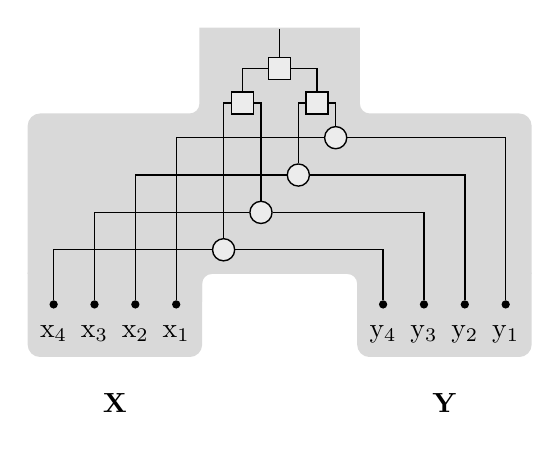
\begin{tikzpicture}
% background
\path[species background] (0,88.0) -- (0,31.0) -- (62.052,31.0) [sharp corners] -- (62.052,0) -- (119.05199999999999,0) [rounded corners] -- (119.05199999999999,31.0) -- (181.10399999999998,31.0) [sharp corners] -- (181.10399999999998,88.0) [rounded corners] -- (119.05199999999999,98.0) -- (119.05199999999999,88.0) -- (62.052,88.0) [sharp corners] -- (62.052,98.0) -- cycle;
\path[species background] (0,88.0) -- (0,118.0) -- (62.052,118.0) -- (62.052,88.0);
\path[species background] (119.05199999999999,88.0) -- (119.05199999999999,118.0) -- (181.10399999999998,118.0) -- (181.10399999999998,88.0);
% species
\path[species border] (0,88.0) -- (0,31.0) -- (62.052,31.0) -- (62.052,0);
\path[species border] (181.10399999999998,88.0) -- (181.10399999999998,31.0) -- (119.05199999999999,31.0) -- (119.05199999999999,0);
\path[species border] (62.052,88.0) -- (62.052,88.0) -- (119.05199999999999,88.0) -- (119.05199999999999,88.0);
\path[species border] (0,88.0) -- (0,118.0) -- node[species label] {X} (62.052,118.0) -- (62.052,88.0);
\path[species border] (119.05199999999999,88.0) -- (119.05199999999999,118.0) -- node[species label] {Y} (181.10399999999998,118.0) -- (181.10399999999998,88.0);
% gene branches
\draw[branch={reccolor0}] (53.170500000000004,88.0) |- (106.55199999999999,39.25) (115.05199999999999,39.25) -| (172.2225,88.0);
\draw[branch={reccolor0}] (38.4075,88.0) |- (93.05199999999999,52.75) (101.55199999999999,52.75) -| (157.4595,88.0);
\draw[branch={reccolor0}] (110.80199999999999,35.0) |- (99.80199999999999,26.75) (108.30199999999999,26.75) -| (97.30199999999999,48.5);
\draw[branch={reccolor0}] (23.6445,88.0) |- (79.55199999999999,66.25) (88.05199999999999,66.25) -| (142.6965,88.0);
\draw[branch={reccolor0}] (8.881500000000003,88.0) |- (66.05199999999999,79.75) (74.55199999999999,79.75) -| (127.93349999999998,88.0);
\draw[branch={reccolor0}] (83.80199999999999,62.0) |- (72.80199999999999,26.75) (81.30199999999999,26.75) -| (70.30199999999999,75.5);
\path[branch={reccolor0}] (90.55199999999999,10.0) -- (90.55199999999999,0);
\draw[branch={reccolor0}] (104.05199999999999,22.5) |- (86.30199999999999,14.25) (94.80199999999999,14.25) -| (77.05199999999999,22.5);
\path[branch={reccolor0}] (53.170500000000004,98.0) -- (53.170500000000004,88.0);
\path[branch={reccolor0}] (38.4075,98.0) -- (38.4075,88.0);
\path[branch={reccolor0}] (23.644499999999997,98.0) -- (23.6445,88.0);
\path[branch={reccolor0}] (8.881499999999999,98.0) -- (8.881500000000003,88.0);
\path[branch={reccolor0}] (172.22249999999997,98.0) -- (172.2225,88.0);
\path[branch={reccolor0}] (157.45949999999996,98.0) -- (157.4595,88.0);
\path[branch={reccolor0}] (142.6965,98.0) -- (142.6965,88.0);
\path[branch={reccolor0}] (127.9335,98.0) -- (127.93349999999998,88.0);
% gene transfers
% events
\node[speciation={reccolor0}] at (110.80199999999999,39.25) {};
\node[speciation={reccolor0}] at (97.30199999999999,52.75) {};
\node[duplication={reccolor0}] at (104.05199999999999,26.75) {};
\node[speciation={reccolor0}] at (83.80199999999999,66.25) {};
\node[speciation={reccolor0}] at (70.30199999999999,79.75) {};
\node[duplication={reccolor0}] at (77.05199999999999,26.75) {};
\node[duplication={reccolor0}] at (90.55199999999999,14.25) {};
\node[extant gene={reccolor0}{x\textsubscript{1}}] at (53.170500000000004,99.5) {};
\node[extant gene={reccolor0}{x\textsubscript{2}}] at (38.4075,99.5) {};
\node[extant gene={reccolor0}{x\textsubscript{3}}] at (23.644499999999997,99.5) {};
\node[extant gene={reccolor0}{x\textsubscript{4}}] at (8.881499999999999,99.5) {};
\node[extant gene={reccolor0}{y\textsubscript{1}}] at (172.22249999999997,99.5) {};
\node[extant gene={reccolor0}{y\textsubscript{2}}] at (157.45949999999996,99.5) {};
\node[extant gene={reccolor0}{y\textsubscript{3}}] at (142.6965,99.5) {};
\node[extant gene={reccolor0}{y\textsubscript{4}}] at (127.9335,99.5) {};
\end{tikzpicture}
